\documentclass[titlepage]{article}

\usepackage{amsmath}
\usepackage{amsfonts}
\usepackage{graphicx,picture,calc}
\usepackage{tikz}
\usepackage{url}
\usepackage{subfig}
\linespread{2}
\usepackage{float}

\usepackage{epsfig}

\usepackage{lineno}
\linenumbers

\usepackage[affil-it]{authblk}

\usepackage{natbib}
\bibliographystyle{mee}
\bibpunct{(}{)}{;}{a}{}{;}

\usepackage{soul}
\usepackage{gensymb}

%opening
\title{Using Balanced Acceptance Sampling as a master sample for environmental surveys}
%\author{Paul van Dam-Bates, Oliver Gansell, \& Blair Robertson}

\author[1,*]{Paul van Dam-Bates}
\author[2]{Oliver Gansell}
\author[3]{Blair Robertson}

\affil[1]{%
	Planning Monitoring and Reporting, Department of Conservation, Christchurch, New Zealand 
}
\affil[2]{%
	Planning Monitoring and Reporting, Department of Conservation, Hamilton, New Zealand}

\affil[3]{%
	School of Mathematics and Statistics, University of Canterbury, Christchurch, New Zealand}

\affil[*]{Corresponding author: Paul van Dam-Bates, paul.vandambates@gmail.com}


\begin{document}

\maketitle


\begin{abstract}
Well designed environmental monitoring programmes for management organisations are important for evidence based decision making. However, many environmental problems are not single agency, single spatial scale issues. A master sample can be used to coordinate and scale monitoring designs to ensure consistency in information gathered and robustness of estimators at the different spatial scales. We propose using Balanced Acceptance Sampling (BAS) to generate a master sample. Using BAS as a master sample is flexible, effective and improves on other methods previously explored. Some practical aspects of the design are addressed such as inclusion of legacy monitoring programmes, stratification, unequal probability sampling, rotating panel designs, and regional intensification. An example master sample is presented for environmental monitoring in New Zealand.

\end{abstract}

{\bf Keywords:} Master Sample, Spatial Balance, Environmental Monitoring, Legacy Monitoring.

\section{Introduction}
Environmental management agencies rely on the results of monitoring to answer questions about the success of their policies and programmes. Monitoring is often designed to address information needs for a particular site or small set of sites. If the study is poorly designed it can result in failure to provide meaningful data to inform management and policy decision making \citep{Legg2006, Nichols2006, Field2007}. Extrapolating from these studies to answer larger scale questions can bias the estimates as single sites are rarely representative of a broader region \citep{dixon1998measuring, Peterson1999}.

Increasingly, monitoring on a large scale is needed to inform management needs and assess progress towards targets concerned with changes in biodiversity globally \citep{noss1999assessing, buckland2005monitoring, pereira2006towards, magurran2010long}. The monitoring objectives and the sample area between the national, regional, and local agencies often overlap creating efficiencies if the different groups coordinate their effort. Coordinating requires consistent formulation of goals and objectives, selection of indicators and measures, field protocols and sample design \citep{LarsenOlsenStevens2008, fancy2009monitoring, Reynolds2016}. If one agency establishes monitoring locations using standard methods and sample design, another agency can use that data for their own purposes, reducing the need to establish more monitoring. By agencies working together and through a well set out design process, as described in \citet{Reynolds2016}, the chances of monitoring being successful are higher and concerns about extrapolating estimates from disparate data sources is also reduced.

One way to coordinate sample design is to develop a master sample; a set of points that can be sub-sampled for different monitoring activities. This was first proposed by \citep{King1945}, but only recently has been introduced to environmental monitoring \citep{LarsenOlsenStevens2008, theobald2016} with implementation in the Pacific Northwest of the United States. Having different studies draw samples from the master sample has the benefit of enhancing collaboration within and between agencies to reduce duplication of effort. Additionally, consistent sample design has benefits when making estimates using data from multiple sources. Similar to providing standard field methods, the master sample provides standardised locations for sampling that ensures objective, unbiased estimation of the population parameters of interest. This coordination reduces convenience or judgement sampling and requires the user to define the objectives and sample frame clearly before gaining access to the sample points. 

The sampling method chosen should be flexible enough for a variety of users and study designs to be effective for coordination. Monitoring can take place on different spatial scales such as a national monitoring programme or a local one, investigating the impact of management action. When designing an individual study, identifying heterogeneity and using stratification \citep{Yoccoz2001} or unequal probability sampling \citep{Stevens1997} can produce more precise estimates. The study may need a unique balance of status and trend estimation which can be done by defining panels that have different revisit schema \citep{Skalski1990, StevensOlsen1999, Mcdonald2003}. In all these cases the sub-samples used should be unbiased and representative.

There are many ways to generate effective samples which could be used to coordinate monitoring. A simple random sample is unbiased but is less efficient than spatially balanced designs in the presence of spatial autocorrelation \citep{cochran1946relative, Grafstrom2013}. A design is spatially balanced if the sample is well-spread over the population --- a sample with few clumps and voids. A systematic sample can be considered near perfect spatial balance but is less flexible to changes in sample size making it a poor choice. \citet{StevensOlsen2004} introduced Generalised Random Tessellation Stratified (GRTS) design, a spatially balanced design that is frequently used in environmental monitoring. GRTS hierarchically orders a population using a base four numbering scheme and then selects a systematic sample from the ordered population. There is also the Local Pivotal Method (LPM) \citep{Grafstrom2012}. LPM iteratively updates each sampling unit's inclusion probability in a way that makes it very unlikely to include neighbouring units in a sample. Once $n$ units have an inclusion probability of one, the sample is released. Although the spatial balance of LPM is better than GRTS, it is computationally prohibitive on large populations. For large populations, \citet{Grafstrom2014} introduced a new rapid implementation of LPM, called suboptimal LPM. LPM has better spatial balance, but suboptimal LPM is computationally feasible on large populations. Another spatially balanced design is Balanced Acceptance Sampling (BAS) \citep{Robertson2013}. It uses a quasi-random number sequence to generate spatially balanced points. Similar to GRTS, the outcome of the sequence is an ordered set of points such that any contiguous sub-sample maintains spatial balance.

GRTS has been used to generate environmental monitoring master samples \citep{LarsenOlsenStevens2008}. The design is particularly useful for generating master samples because GRTS points are ordered using a reverse hierarchical ordering strategy that ensures that all contiguous sub-samples are also spatially balanced \citep{StevensOlsen2004}. By taking a large GRTS oversample, an ordered master sample can be obtained from which spatially balanced sub-samples can be drawn. However, once an oversample is chosen, it is not possible to generate additional points and this needs to be accounted for at the planning stage. \citet{theobald2016} also uses an adaptation of GRTS, Reversed Randomized Quadrant-Recursive
Raster (RRQRR), implemented in ArcGIS software \citep{theobald2007} to coordinate monitoring effort. The authors' are not aware of an ordering strategy for the LPM methods and hence, it is not clear how these methods could be used for oversampling. BAS, similar to GRTS, creates an ordered set of points such that any contiguous sub-sample maintains spatial balance. To generate a master sample with BAS, a random-start is chosen and after that an infinite set of points exist for the sample. Hence, the oversample size does not need to be specified.

The purpose of this paper is to develop a master sample for environmental monitoring with a focus on terrestrial sampling of an area frame in which all sub-samples have positive area. We investigate using BAS to generate a master sample; how the points will be generated and then used in a wide variety of ways. These include adapting to different spatial scales, stratification and unequal probability sampling, changes in boundaries or resources, revisitation structure (panel design), and how to include legacy monitoring programmes. We then provide an example for how this could be applied to coordinate biodiversity monitoring at the regional and national level in New Zealand.

\section{Methods}
\subsection{Point selection}

Two-dimensional BAS points are drawn from a random-start Halton sequence $\{{\bf x}_k\}_{k=1}^{\infty} \subset [0,1)^2$. The $i$th coordinate of each point in the sequence has an associated base $b_i$, with $b_1 = 2$ and $b_2 = 3$. The $i$th coordinate of the $k$th point in this sequence is (Robertson et al.\ 2017)
$$
x_k^{(i)} = \sum_{j = 0}^{\infty} \left\{\left\lfloor \frac{u_i + k}{b_i^j} \right\rfloor \text{ mod } b_i \right\}\frac{1}{b_i^{j+1}},
$$
where $u_i$ is a random non-negative integer and $\lfloor x \rfloor$ is the floor function --- the largest integer that is less than or equal to $x$. For example, the first coordinate of the second point with $u_i = 1$ and $b_i = 2$ is

\begin{eqnarray*}
x^{(1)}_{2} & = & \left(\left\lfloor \frac{3}{1} \right\rfloor \text{ mod } 2 \right)\frac{1}{2} + \left(\left\lfloor \frac{3}{2} \right\rfloor \text{ mod } 2 \right) \frac{1}{4} +\left(\left\lfloor \frac{3}{4} \right\rfloor \text{ mod } 2 \right) \frac{1}{8}\\
& = & \frac{1}{2} + \frac{1}{4} + 0\\
& = & \frac{3}{4}.
\end{eqnarray*}

\noindent The two-dimensional random-start Halton sequence is 
\begin{equation}\label{BASeq}
\{{\bf x}_k\}_{k=1}^{\infty} = \left\{x_k^{(1)}, x_k^{(2)}\right\}_{k=1}^{\infty}.
\end{equation}
Setting $u_1 = u_2 = 0$ gives the classical two-dimensional Halton sequence \citep{Halton1960}. 

The points from eqn \ref{BASeq} are scaled to a minimal bounding box enclosing the study area and the first $n$ scaled points in the study area define the BAS sample. The BAS points are kept in the same order as they appear in eqn \ref{BASeq} and will have good spatial spread over the study area. Furthermore, any continuous subset of the BAS sample will also have good spatial spread \citep{Robertson2017}.

The random integer vector in the sequence ${\bf u} = (u_1, u_2) \in [0,10^7]^2$ is chosen so that ${\bf x}_1$ falls within the sample area \citep{Robertson2017}. This gives $\lambda 10^{14}$ possible BAS samples of size $n$, where $\lambda$ is the fraction of the bounding box occupied by the study area. By ensuring the random start comes from a large set of integers, the BAS points are uniformly distributed \citep{Robertson2013}. Once the random-start is selected an infinite number of BAS points exist over the study which constitutes the master sample. Higher dimensional points can be defined by using different co-prime bases for each additional dimension (e.g. $b_3 = 5$ when sampling from a $[0,1)^3$).

\subsection{Spatial Scales}
The master sample should work at different spatial scales to answer national, regional, and local objectives. Let $A$ be a measurable subset of the study area for which the master sample is defined. Because the master sample $\{{\bf x}_k\}_{k=1}^{\infty}$ is uniformly distributed over $[0,1)^2$ \citep{Wang2000} and $A$ is measurable, there exists a subsequence $\{{\bf z}_j\}_{j=1}^{\infty} \subset \{{\bf x}_k\}_{k=1}^{\infty}$ such that each ${\bf z}_j \in A$. Furthermore, $\{{\bf z}_j\}_{j=1}^n$ is a BAS sample of size $n$ drawn from $A$, with its random start and bounding box defined by the master sample. Hence, BAS samples can be drawn from the master sample at any spatial scale within the study area of the master sample. This also means that a national sample can share points with monitoring at the local level (see Section 2.4).

\subsection{Stratification and Unequal probability}
Stratification with the master sample is essentially the same as taking a sub-sample for a specific measurable subset of the study area as described above. The $i$th stratum (measurable) has a subsequence $\{{\bf z}_j\}_{j=1}^{\infty} \subset \{{\bf x}_k\}_{k=1}^{\infty}$ such that each ${\bf z}_j$ is in the stratum. The BAS sample for the $i$th stratum is $\{{\bf z}_j\}_{j=1}^{n_i}$, where $n_i$ is the sample size required. Hence, each stratum has its own BAS sample with its random start and bounding box defined by the master sample.

If unequal probability sampling is required, a third dimension is added to the bounding box. This extra dimension allows BAS to sample from an arbitrary inclusion density function $\pi(\bf{x})$ using an acceptance/rejection sampling strategy \citep{Robertson2013}. Specifically, a point ${\bf x}_k = (x_k^{(1)}, x_k^{(2)}, x_k^{(3)})$ is accepted if $(x_k^{(1)}, x_k^{(2)})$ is in the study area and $\pi(x_k^{(1)}, x_k^{(2)}) \leq \alpha x_k^{(3)}$, where $\alpha$ is a scaling factor to ensure $\max_{{\bf x}}\pi({\bf x}) = 1$. The impact of this is that some of the master sample points in eqn(\ref{BASeq} will be skipped. Skipping points in eqn \ref{BASeq} changes the distribution of points in each BAS sample, with fewer points being drawn from areas where $\pi({\bf{x}})$ is low.

\subsection{Changing boundaries and resources}
For long-term monitoring programmes, the boundaries of study regions may change over time. This is easy to accommodate with the master sample, provided the changes are within the initial bounding box. Let $A$ be a measurable study area whose boundaries changed, defining a new measurable study area $B$ with $A \cap B \neq \emptyset$. If there are no sampled BAS points in $A \cap B$, points from the master sample are drawn to sample $B$. Otherwise, let ${\bf x}_k$ be the sampled point in $A \cap B$ with the largest index $k$. A BAS sample in $B$, that includes sampled points from $A \cap B$, is achieved if all the master sample points that fall in $B$ with indices less than $k$ are sampled. If a smaller sample is desired in $B$, potentially due to a change in resources, then points with the larger indices in $B$ are removed (See Figure \ref{CB}). If more points are required, then points can be added from the master sample in $B$ until the new sample size is achieved. Ensuring that BAS samples are drawn from each study region means that spatial balance and good sampling properties are maintained.

\subsection{Panel design}
In environmental surveys that are repeated through time, some samples may be visited more frequently than others. Estimates of status and/or trend can be improved by balancing the number of new points sampled each year with repeated sampling on existing points \citep{Urquhart1999}. A panel is defined as all samples that have the same visitation schedule. The points within a panel as well as between panels should be representative and unbiased. A panel design is achieved using the master sample by choosing the subset of points $\{{\bf z}_j\}_{j=1}^{\infty}$ that fall within the the study area and the order of the points define each panel. For panel 1 we use $\{{\bf z}_j\}_{j=1}^{n_1}$, for panel 2 we use $\{{\bf z}_j\}_{j=1 + n_1}^{n_1 + n_2}$ and so on, where $n_i$ is the sample size for the $i$th panel. By defining the panels this way the overall sample is still a BAS design as well each panel. Once a full rotation of all samples has been carried out, if additional points are needed, they are added from the unsampled points in the master sample in the order that they appear. Note, when this occurs each panel may not be a true BAS sample but as shown in the legacy units simulation below, adding BAS points to an existing sample does not significantly impact estimation and the sample will still be equi-probable and give unbiased estimators. If budgets change, points should be removed by last in, first out. Table \ref{Panel} shows an example panel design.

\subsection{Incorporating legacy monitoring}
A master sample is intended for coordinating large scale monitoring. Often, there is legacy monitoring that may already be well designed and this should be accommodated. We will consider two different types of legacy monitoring designs: simple random sampling (SRS) and random-start systematic sampling (SS). These are equi-probable designs, where each sampling unit has an equal chance of being included in a sample. If the existing monitoring is insufficient, the BAS master sample can be used to draw additional units from the area. Furthermore, the inclusion probabilities around the legacy units can be decreased to reduce the chance of drawing units close to the legacy units \citep{Foster2017}. Using the unequal probability sampling method described above, we can incorporate this method into the master sample. We will call the altered inclusion probability sampling method aBAS.

For unbiased estimation, inclusion probabilities need to be specified. Using an existing $n_l$ legacy units and augmenting with $n_b$ BAS units from a population of $N$ units, we assume the legacy units have equal inclusion probabilities $\pi_l = (n_l + n_b)/N$. The inclusion probabilities for the remaining units are then specified by the user so $\sum_{i = 1}^{N} \pi_i = n_l + n_b = n$. For example, an equi-probable design uses $\pi_i = (n_l + n_b)/N$ for $i = 1,2,..., N$. By making an assumption about the legacy monitoring and generating BAS points independently, the design and analysis is simple. However, incorporating legacy units this way may decrease the overall spatial balance of the sample which in the presence of strong spatial autocorrelation can impact precision and is why aBAS has better precision \citep{Foster2017}.

Spatially balanced designs use a local neighbourhood variance (LNV) \citep{StevensOlsen2003} and as the proportion of legacy units is increased the LNV underestimates true variance \citep{Foster2017}. If the legacy units and the augmented samples are considered separately with sample size $n_l$ and $n_b$ ($n_l + n_b = n$) respectively, then the mean can be written as  

\begin{equation}
\hat{y} = \frac{n_l}{n}\sum_{i = 1}^{n_l}\frac{y_l}{N \pi_{li}^*} + \frac{n_b}{n}\sum_{i = 1}^{n_b}\frac{y_b}{N \pi_{bi}^*}
\end{equation} 

\noindent where the inclusion probabilities are rescaled $\pi_{li}^* = \pi_{i} \times \frac{n}{n_l}$ and $\pi_{bi}^* = \pi_{i} \times \frac{n}{n_b}$. It then follows that the variance can be estimated as

\begin{equation}\label{VAReq}
\widehat{\text{var}}(\hat{y}) = \left(\frac{n_l}{n}\right)^2 \times \widehat{\text{var}}(\hat{y}_l) + \left(\frac{n_b}{n}\right)^2 \times \widehat{\text{var}}(\hat{y}_b).
\end{equation}

\noindent Here $\widehat{\text{var}}(\hat{y}_l)$ is the Sen, Yates and Grundy variance estimate using the legacy units and $\widehat{\text{var}}(\hat{y}_b)$ is the LNV variance estimate using spatially balanced units. 

A simulation study was carried out to investigate the different methods to incorporate legacy monitoring. The sampling frame was defined as a $100\times100$ raster in $[0,1)^2$ and an estimate of the population mean and standard error was sought. The response value for each raster cell was defined as the integral of $f(\boldsymbol{x})$ over the cell. Three different functions were considered, a strong spatial trend \citep{Robertson2013, Grafstrom2012}, the Peak function, and the Bird function. These functions are given in the online supplementary material section. Scenarios similar to \citet{Foster2017} using the program R \citep{R} were run. We used an overall sample size of $n = 60$. A number of legacy units $(n_l \in 3,4,...,57)$ were generated either as SRS or SS. More units $(n_b = 60 - n_l)$ were generated using GRTS \citep{spsurvey}, BAS, aBAS \citep{MBHdesign} and SRS to achieve the full sample size of $n = 60$. Each scenario was run 1000 times. When estimating the standard error of SS units we assumed a simple random sample, which provides conservative estimates in the presence of spatial autocorrelation \citep{Lundberg2014,Strand2017}. A detailed description of the simulation and functions used can be accessed in the supplementary material.

The results of the simulation can be seen in Figure \ref{estimation}. In all cases, adding some spread to the points improved precision over using SRS. aBAS performed the best when SRS legacy units were used, but had similar performances to BAS and GRTS for SS. The SS legacy units already had good spread and aBAS was not necessary to force better overall spatial balance. Population 3 has periodic structure, which made systematic sampling perform poorly because the spread of the legacy units matched the structure of the population. The standard error estimate from eqn \ref{VAReq} was relatively accurate for SRS, although conservative for aBAS and overestimated as expected for SS. The legacy monitoring was improved by augmenting the samples with spatially balanced points. Given that the legacy monitoring is well designed, there are no issues with incorporating legacy samples with the master sample.

We recommend using aBAS for single measurements or simple repeated studies when legacy monitoring is SRS or poorly spread. However, it is important that inclusion probabilities are positively correlated to the response variable \citep{Robertson2017} and this is not the case for ordered subsets of aBAS. As a result, a rotating panel design may lose precision using aBAS when legacy units are not sampled on each occasion. For estimation with aBAS we assumed equal inclusion probabilities which is only met when the sample is made up of a single equi-probable random legacy sample followed by a single aBAS sample. Multiple samples of aBAS on the same legacy units would violate this as well as any issues in the process for how the legacy monitoring was designed. In general, we recommend to generate spatially balanced points independently of the legacy monitoring and combine the two methods only when the legacy monitoring is well designed. For design-based estimation, the variance estimate in eqn \ref{VAReq} should be used. This corrects the underestimation of LNV but requires there are four or more spatially balanced points as suggested in the spsurvey package in R \citep{spsurvey} and three or more legacy points. Otherwise, use LNV ($n_l < 3$) or the legacy variance estimator ($n_b < 4$) for all points. In practice, model-based estimation is often used and any analyses should account for the spatial aspect of the design as in \citet{Foster2017}.

\section{Application: New Zealand terrestrial monitoring}
The New Zealand Department of Conservation (DOC) is the lead biodiversity management agency in New Zealand (NZ), responsible for managing $\approx 30\% $ of New Zealand as public conservation land (PCL). Development of a national monitoring system has exposed the challenges in coordinating monitoring design to provide results meaningful at a local, regional and national scale. Increasingly partner environmental agencies (local government etc.) and central government expect cross-agency collaboration and coordination of systems and processes. Considerable effort has gone into a coordinated approach for indicators and measures and field protocols \citep{DOC}. There is an existing national sample of PCL, known as the National Level Monitoring (NLM) programme which is an 8-km systematic grid of $\approx 1400$ monitoring sites \citep{Coomes2002}. The NLM programme focusses on status and trend monitoring at the national scale of key indicators of ecosystem structure and composition. Through ongoing collaboration with local government agencies, the grid has been extended off PCL.

DOC ecosystem and species management is focussed on a suite of priority sites known as Ecosystem Management Units (EMUs). To assess the outcome of management interventions across all EMUs, the 8-km grid NLM needs to be intensified with changes to visitation frequency and methods relating to the specific management monitoring objectives. At the same time, there are EMU specific questions to be answered that require another intensification to a regional/local level. For example, one of DOC's EMUs, Abel Tasman National Park (ATNP) (40\degree56'03.8''S 172\degree58'19.7''E), is managed in partnership with a philanthropic foundation. The agreement governing this partnership requires the foundation to invest in the recovery of biodiversity in ATNP. Once it is shown that the targets pertaining to increases in the abundance and distribution of bird species and vegetation condition are met, DOC will be responsible for the maintenance of biodiversity in ATNP. Monitoring is required to establish the current state of key indicators in ATNP and then determine when agreed targets have been achieved. A sample design is required which can incorporate the existing NLM monitoring, sample broad scales and enable local intensification of monitoring.

A national sample of New Zealand using BAS can make up the master sample, with the existing NLM points included. For efficiency and simplicity, each island (North Island, South Island, Stewart Island, Chatham Islands, etc.) will be stratified and have their own bounding box and random seed. The seed chosen for the South Island was ${\bf u} = (4887260, 18041662)$ with minimum bounding box in New Zealand Transverse Mercator 2000 (NZTM2000)

$$
[1089354, 1721164] \times [4747979, 5516919].
$$
These values define the scaling needed to map the random start Halton points to the South Island of New Zealand (NZ). For example, the first point is
\begin{eqnarray*}
	{\bf x}_1 & = & (631810 x_1^{(1)} + 1089354, 768940 x_1^{(2)} + 4747979)\\
	& \approx & (1235673, 5075613).
\end{eqnarray*}

To sample EMUs in NZ using the master sample, select all sites that fall within EMU polygons. The actual required sample size and visitation frequency should reflect the monitoring objectives and follow a similar process as outlined by \citep{Reynolds2016}. See Figure \ref{EMU} for an example of clipping the master sample on the South Island into the first 500 samples that fall within EMUs.

At ATNP, one of the key targets is focussed on bird abundance and distribution through the park. A sample size of $n = 65$ was chosen based on a precision analysis using simr \citep{simr} and historical bird count data from an existing intensively monitored site which showed that temporal variation was less than spatial. Therefore, 15 samples were selected to be measured annually and the other 50 on a rotating 5-year panel $[1-0,(1-4)^5]$. From the NLM programme mentioned above, there were four legacy samples in the sample frame which would be included in the rotating panel on years corresponding to the years they are to be sampled. If DOC implemented an EMU monitoring programme of 500 augmented points on the South Island, then there would be an additional seven points in ATNP monitored and funded by DOC using the master sample. The EMU points would make up Panel 1 based on the hierarchical order of the master sample. See Figure \ref{Tasman} for the selected points in this monitoring programme. ATNP is an example of localised monitoring using the master sample that can contribute to national estimates of bird abundance and distribution. DOC gets better precision with the increased sampling in ATNP and the philanthropic foundation saves resources by using DOC's national investment in monitoring explicitly in their design.

The master sample above is entirely defined by the seed ${\bf u}$ and the bounding box. Hence, there is no need for a repository to hold the coordinates. Computationally the master sample is easy to run on the fly. Generating 65 points for ATNP in Figure \ref{Tasman} takes $\approx 0.5$ seconds on a desktop computer. See supplementary materials for R script to generate a master sample in New Zealand.

\section{Discussion}
A master sample can be a useful tool to organise environmental monitoring at different spatial scales as previously done using GRTS or RRQRR \citep{LarsenOlsenStevens2008, theobald2016}. By using BAS instead of GRTS there is better spatial balance \citep{Robertson2013} and no need for an oversample. It is also possible to add an extra dimension to do unequal probability sampling leading to an overall more flexible design. Depending on the population being sampled, spatial balance may or may not lead to a more precise sample than simple random sampling. However, it is likely that some spatial balance will improve efficiency for most designs. Not needing to oversample to create a master sample using BAS means that it will remain relevant at any scale that monitoring takes place no matter how localised. BAS can be used for sampling three-dimensional space \citep{Robertson2013} which generalises the concepts presented here to work for atmospheric or oceanic monitoring. 

Previous master samples rely on large source files for point coordinates. BAS does not because it is deterministic once the random seed is chosen. Generating a BAS master sample in R is computationally quick and easy to program making it possible for a user to run a function in R (see supplementary online material section) to sample a chosen region from a shape file. Note, by making use of the deterministic nature of the Halton sequence and Halton boxes \citep{Robertson2017} the code can be made computationally efficient for any set of shape files and sample sizes required.

In our experience, any large scale long-term monitoring will need to incorporate already existing monitoring programmes that are proven effective. This was a requirement in developing a master sample for New Zealand. We have shown that there is no major issue with incorporating legacy monitoring into the design but recommend that all sites are rigorously vetted to ensure no known biases are included if historically the sites were judgement samples or for other reasons. Using panel designs can help incorporate the already existing visitation schedule of the legacy sites into an efficient monitoring design. By generating the master sample independently of the legacy monitoring it is possible that a legacy site and master sample site could be close, in this case both sites still need to be sampled.

The master sample helps coordinate the points sampled for environmental surveys. Every survey at the local and national level should still go through rigorous design. This means defining the objectives of monitoring clearly and the methods to use so that they are consistent with standard methodology as required by the objective. By following the steps outlined in \citet{Reynolds2016} and using the master sample for point generation, we believe that the monitoring programmes undertaken at all levels will have improved efficiency and contribute to the overall knowledge of the population of interest.

\section{Acknowledgements}
This research was funded by the Department of Conservation in New Zealand. We would like to thank Elaine Wright for her support, Tony Olsen, Scott Foster and Amy Hawcroft for their advice.

\bibliography{MasterSampleLit}	

\section{Supporting Information}
More information about the simulation study and the R code used to generate the Master Sample for New Zealand can be found in the supplementary text.

\section{Data Availability}
We present a maintained version of the R code to generate a master sample in New Zealand, including a shape file example on github for access to readers familiar with R. \url{https://github.com/ogansell/MSampNZ}.

\section{Author Contribution}
All authors had significant contributions to this research. The paper was initiated by a requirement from the Department of Conservation (DOC) for coordinated monitoring of ecosystems at the national level. This work fell directly to Ollie Gansel and Paul van Dam-Bates who collaborated with Blair Robertson. We were funded as salary through our roles at DOC and the University of Canterbury.

\newpage
\section*{Figures and Tables}
%This is where we will keep all figures.

\begin{table}[H]
	\caption{Example of a panel design in which panel 1 is sampled annually and panels 2-4 are sampled with a 2 year break in between described as $[1-0,(1-2)^3]$ in \citet{Mcdonald2003}. The sample size $n$ and the points from the master sample in the study area ${\{\bf z_j\}}$ are shown below, where an X indicates that the panel is sampled on that occasion.}
	\begin{tabular}{l l l c c c c c c c c c c }
	\hline
	& & & \multicolumn{10}{c}{Sample Occasion}\\ 
	\cline{4-13}
	Panel & n & Sample & 1 & 2 & 3 & 4 & 5 & 6 & 7 & 8 & 9 & 10 \\ 
	\hline
	1 & 20 & $\{{\bf z_j}\}_{j=1}^{20}$ & X & X & X & X & X & X & X & X & X & X \\
	2 & 10 & $\{{\bf z_j}\}_{j=21}^{30}$ & X &   &  &X &   &   & X &   &  & X \\
	3 & 10 & $\{{\bf z_j}\}_{j=31}^{40}$ &  & X &  &  & X &   &   & X &  &   \\
	4 & 10 & $\{{\bf z_j}\}_{j=41}^{50}$ &  &   &  X  &   &   & X &   &  & X & \\
	\hline
\end{tabular}  
	\label{Panel}
\end{table}

\newpage

\begin{figure}[H]
	\centering
	\subfloat[]{\includegraphics[width=.5\textwidth, angle =-90]{ChangingBoundary1.eps}\label{CB1}}
	\hfill
	\subfloat[]{\includegraphics[width=.5\textwidth, angle =-90]{ChangingBoundary2.eps}\label{CB2}}
	\caption{An example of changing boundaries using a BAS the master sample where each number denotes the index of the BAS point in the master sample. (a) shows 10 points drawn from the master sample in the study region. (b) shows an enlarged region and the 10 points drawn from the master sample in the region. Points 71,77,89 and 95 are removed and 7,25,37 and 52 are included in the new region. If the sample size is increased to 14, then points 61,71,77 and 89 would be included.}\label{CB}
\end{figure}

\newpage

\begin{figure}[H]
	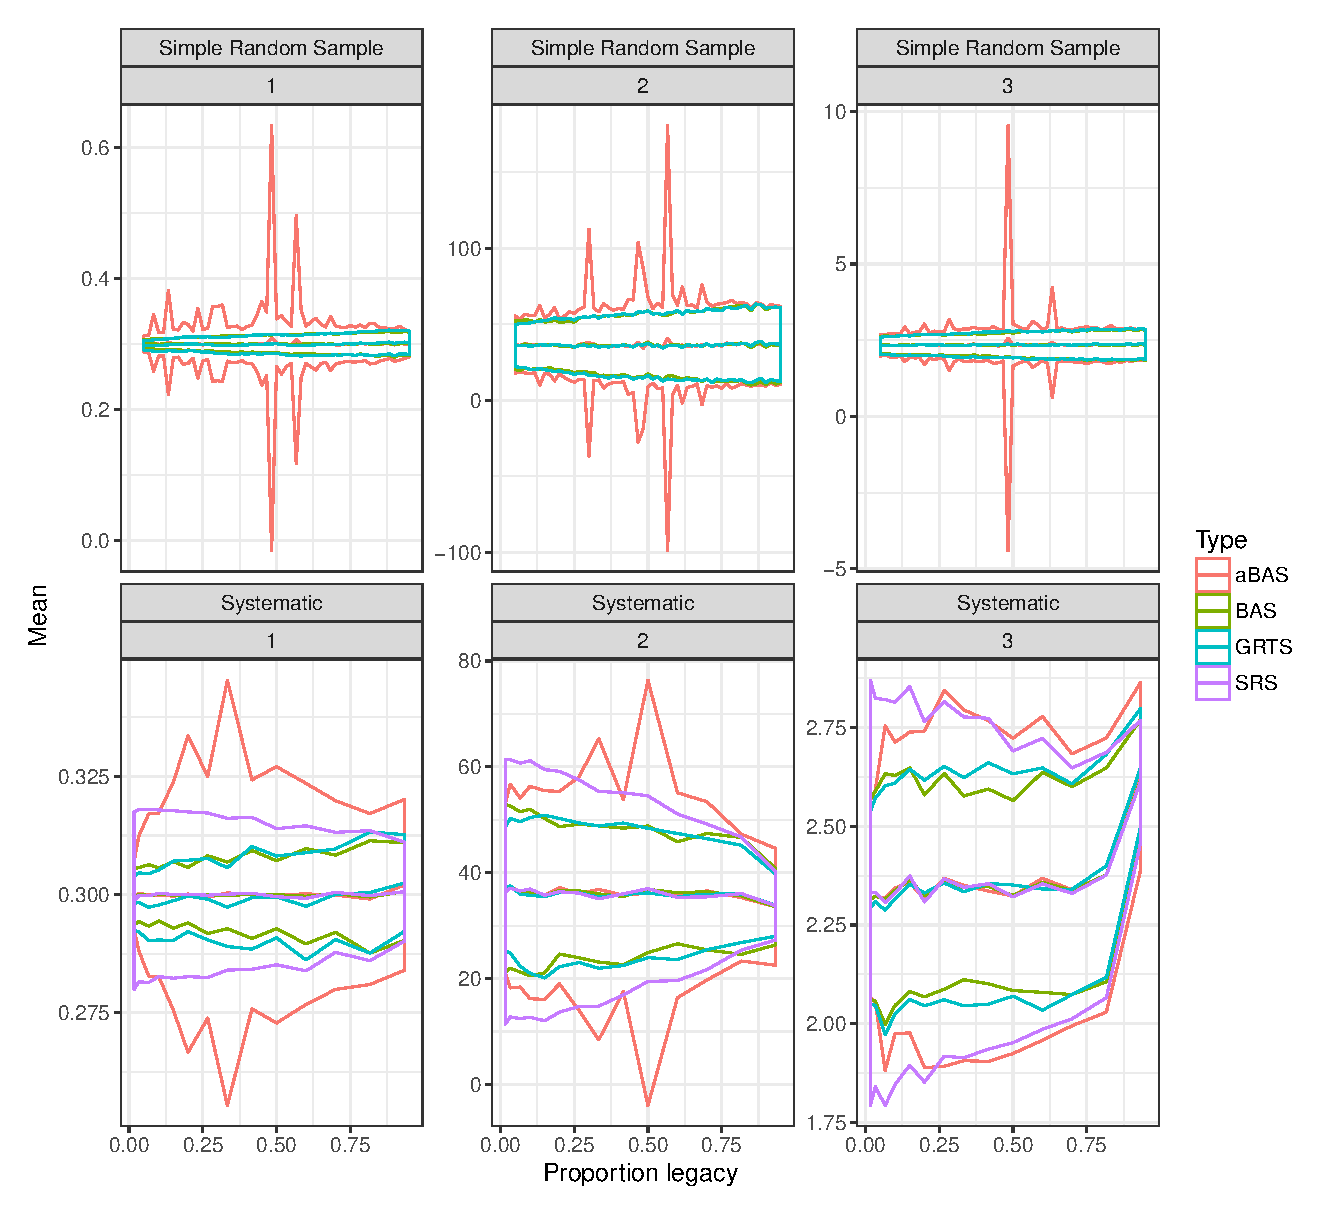
\includegraphics[scale = 0.5]{Estimation.eps}
	\caption{Results from the simulation study testing the impact of adding new samples from altered Balanced Acceptance Sampling (aBAS), Balanced Acceptance Sampling (BAS), Generalised Random Tessellation Stratified (GRTS), and simple random sampling (SRS) to existing legacy monitoring units. Three populations with varying spatial structure were tested. Population 1, a strong spatial trend. Population 2, a peak function. Population 3, a cyclical (bird) function. The estimated and simulated (True) standard errors are shown.}
	\label{estimation}
\end{figure}

\newpage


\begin{figure}[H]
	\centering
	\subfloat[]{\includegraphics[width=0.6\textwidth]{SIMS.eps}\label{NI1}}
	\hfill
	\subfloat[]{\includegraphics[width=0.6\textwidth]{Tier2EMUMS.eps}\label{NI2}}
	\caption{South Island of New Zealand. (a) shows the first 5000 points of the master sample overlayed on red ecosystem management units (EMUs). (b) shows 500 master sample points from (a) that fall within the EMUs in red. Abel Tasman National Park receives seven points which are included as panel 1 points in Figure \ref{Tasman}}
	\label{EMU}
\end{figure}

\newpage

\begin{figure}[H]
	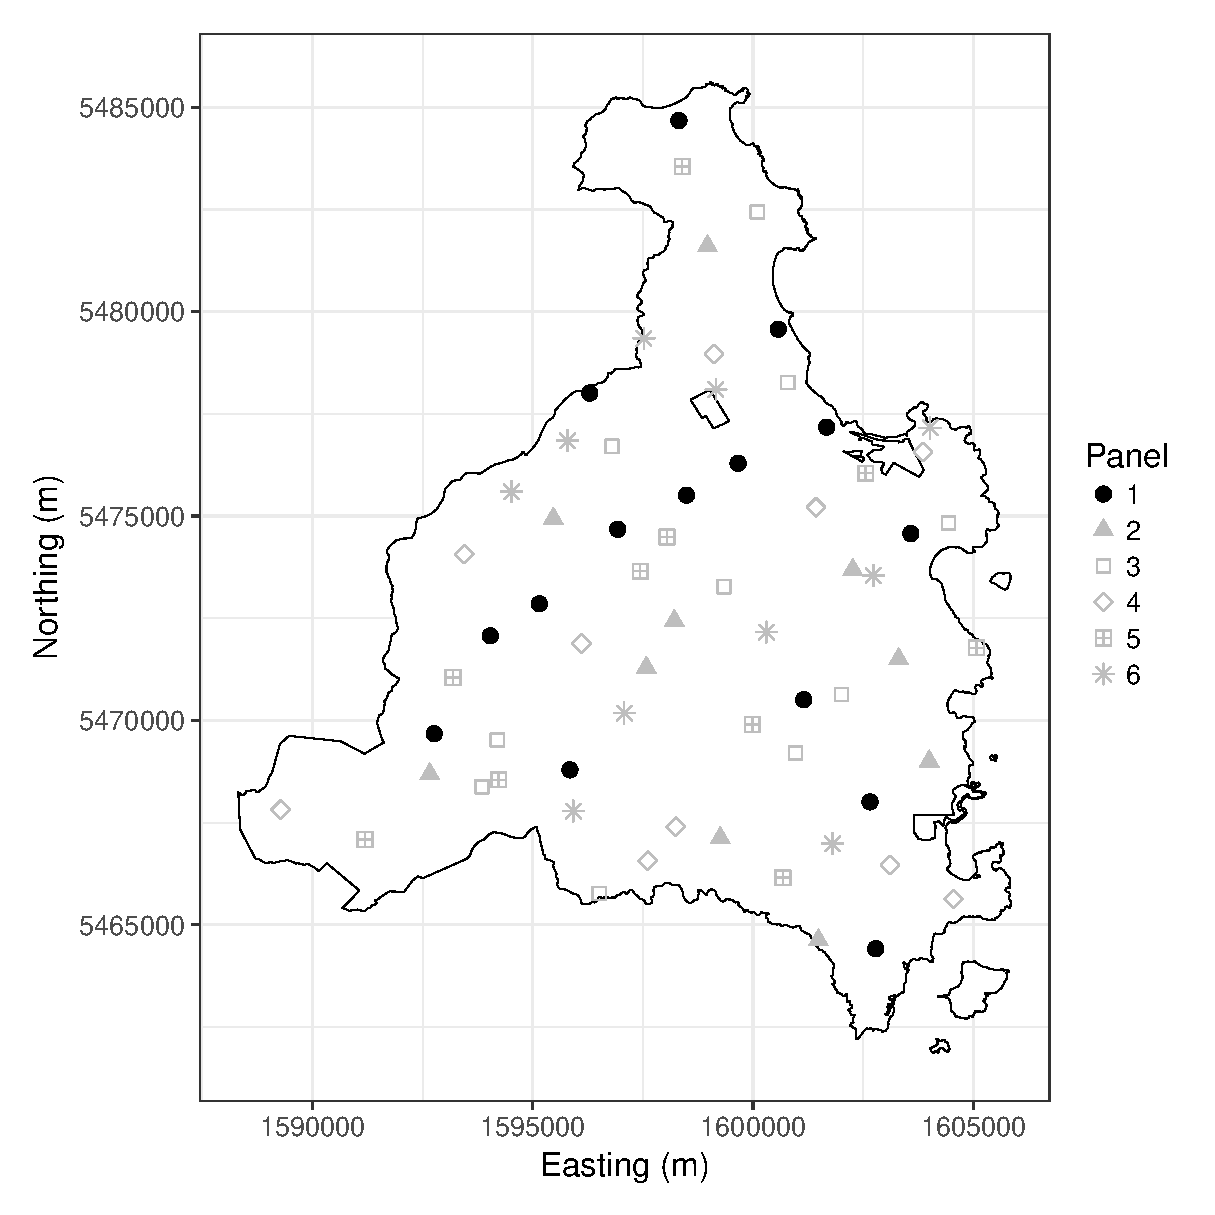
\includegraphics[width = \textwidth]{Tasman.eps}
	\caption{An example of bird monitoring in Abel Tasman National Park New Zealand. Panel 1 is measured annually while the other panels are on a 5-year rotation described as $[1-0,(1-4)^5]$. In the first year, panels 1 and 2 would be measured. Blue points are master sample points measured by a national Ecosystem Management Unit monitoring programme, see Figure \ref{EMU}. The red points are from the 8-km systematic grid National Level Monitoring programme. This design gives excellent spatial coverage over the park each year ($n = 25$) and over a 5-year period ($n=65$).}
	\label{Tasman}
\end{figure}


\end{document}
Old abstract:
Environmental monitoring for management organisations like the Department of Conservation is critical. Without good information about outcomes, poor management actions may persist much longer than they should or initial  intervention may occur too late. The Department currently conducts focused research at key natural heritage sites (Tier 3) as well as a long term national monitoring (Tier 1). The link between the two tiers of investigation to assess the impact of management across New Zealand (Tier 2) is yet to be implemented but faces unique challenges for working at many different spatial scales and coordinating with multiple agencies. The solution is to implement a master sample using Balanced Acceptance Sampling (BAS). To do this some practical aspects of the sample design are addressed such as stratification, unequal probability sampling, rotating panel designs and regional intensification. Incorporating information from Tier 1 monitoring directly is also discussed.